\documentclass[conference]{IEEEtran}
\IEEEoverridecommandlockouts

\usepackage[utf8]{inputenc}
\usepackage[T1]{fontenc}
\usepackage[brazil]{babel}
\usepackage{cite}
\usepackage{amsmath,amssymb,amsfonts}
\usepackage{graphicx}
\usepackage{textcomp}
\usepackage{xcolor}
\usepackage{booktabs}
\usepackage{array}
\usepackage{hyperref}

\hypersetup{
    colorlinks=true,
    linkcolor=blue,
    urlcolor=blue,
    citecolor=blue
}

\begin{document}

\title{Observabilidade e Monitoramento de Recursos do Sistema Operacional com Containers: Estudo Experimental na Plataforma CreateJoy}

\author{
\IEEEauthorblockN{Lívia Gonçalves}
\IEEEauthorblockA{\textit{Dep. de Computação (DECOM)} \\
\textit{CEFET-MG}\\
Belo Horizonte, Brasil}
\and
\IEEEauthorblockN{Nome do Membro 2}
\IEEEauthorblockA{\textit{Dep. de Computação (DECOM)} \\
\textit{CEFET-MG}\\
Belo Horizonte, Brasil}
\and
\IEEEauthorblockN{Nome do Membro 3}
\IEEEauthorblockA{\textit{Dep. de Computação (DECOM)} \\
\textit{CEFET-MG}\\
Belo Horizonte, Brasil}
\and
\IEEEauthorblockN{Nome do Membro 4}
\IEEEauthorblockA{\textit{Dep. de Computação (DECOM)} \\
\textit{CEFET-MG}\\
Belo Horizonte, Brasil}
\and
\IEEEauthorblockN{Nome do Membro 5}
\IEEEauthorblockA{\textit{Dep. de Computação (DECOM)} \\
\textit{CEFET-MG}\\
Belo Horizonte, Brasil}
\and
\IEEEauthorblockN{Nome do Membro 6}
\IEEEauthorblockA{\textit{Dep. de Computação (DECOM)} \\
\textit{CEFET-MG}\\
Belo Horizonte, Brasil}
}

\maketitle

\begin{abstract}
Este trabalho apresenta o projeto, a implantação e o delineamento experimental de uma arquitetura de observabilidade para monitoramento de recursos do sistema operacional hospedeiro e de containers em ambiente orquestrado via Docker Compose. A pilha de coleta e visualização combina Node Exporter, cAdvisor, Prometheus e Grafana para acompanhar utilização de processador (CPU), memória principal (RAM), operações de entrada e saída (I/O) de disco e tráfego de rede. Como sistema alvo, utilizou-se uma instância local isolada da plataforma educacional CreateJoy, executada sobre PHP 8.3 com Apache e banco de dados MariaDB 11.4 populado exclusivamente com registros fictícios. Para induzir contenção de recursos, foram desenvolvidos dois cenários de carga concorrente em Python com a ferramenta Locust: o primeiro simula consultas autenticadas de alunos e solicitações simultâneas na loja interna; o segundo executa envios concorrentes de atividades com arquivos de 1 KB, 100 KB e 5 MB. O documento detalha a topologia de rede, os volumes persistentes, as consultas PromQL provisionadas e a metodologia de validação experimental. Os resultados numéricos e as capturas do Grafana obtidos na execução dos testes de carga encontram-se sinalizados como pendentes de coleta em máquina com Docker ativo.
\end{abstract}

\begin{IEEEkeywords}
Observabilidade, Monitoramento de Recursos, Containers, Docker Compose, Prometheus, Grafana, Contenção de Recursos.
\end{IEEEkeywords}

\section{Introdução}

Aplicações web organizadas em múltiplos serviços compartilham CPU, memória RAM, subsistema de armazenamento e interfaces de rede do sistema operacional (SO) hospedeiro. Sem instrumentação contínua, a degradação de desempenho causada por picos de acessos simultâneos ou por operações intensivas de escrita em disco torna-se difícil de diagnosticar, pois os sintomas percebidos pelo usuário final, como aumento de latência ou erros HTTP, raramente indicam de imediato qual componente atingiu saturação.

O isolamento proporcionado por containers via \textit{namespaces} e \textit{cgroups} do núcleo Linux facilita o empacotamento de serviços, mas não elimina a disputa pelo hardware subjacente. Quando uma aplicação web e seu banco de dados executam no mesmo hospedeiro, requisições concorrentes de leitura, gravação e transferência de arquivos competem por ciclos de processador, largura de banda de rede e filas de I/O. Observar separadamente o consumo do hospedeiro e o consumo individual de cada container permite relacionar eventos da camada de aplicação aos mecanismos de contenção do SO.

Este trabalho tem como objetivo implementar e validar uma infraestrutura reproduzível de observabilidade para a Prática 2 da disciplina de Sistemas Operacionais Modernos, ministrada no Departamento de Computação (DECOM) do CEFET-MG. A solução monitora uma cópia local isolada do sistema de gestão educacional CreateJoy, sem qualquer conexão com o ambiente de produção, integrando métricas de infraestrutura e métricas funcionais da própria aplicação. O restante do texto organiza-se da seguinte forma: a Seção~II descreve a arquitetura de containers, redes e volumes; a Seção~III apresenta o papel técnico de cada ferramenta adotada; a Seção~IV detalha os cenários de carga, os critérios de validação e a análise de contenção de recursos; a Seção~V sintetiza as conclusões e os próximos passos; e a Seção~VI informa o endereço do repositório com todos os manifestos.

\section{Mapeamento da Solução e Arquitetura}

A infraestrutura completa é declarada em um único arquivo \texttt{docker-compose.yml} composto por sete serviços integrados na rede virtual \texttt{monitoring-net}, configurada com o driver \textit{bridge}. A resolução interna de nomes do Docker permite que os serviços se comuniquem diretamente pelos seus identificadores (\texttt{app}, \texttt{db}, \texttt{cadvisor}, \texttt{node-exporter}, \texttt{prometheus}, \texttt{grafana} e \texttt{locust}), dispensando endereços IP estáticos. A Fig.~\ref{fig:arquitetura} ilustra a topologia de rede, o fluxo de coleta de métricas, o direcionamento de carga e o mapeamento dos volumes persistentes.

\begin{figure*}[t]
    \centering
    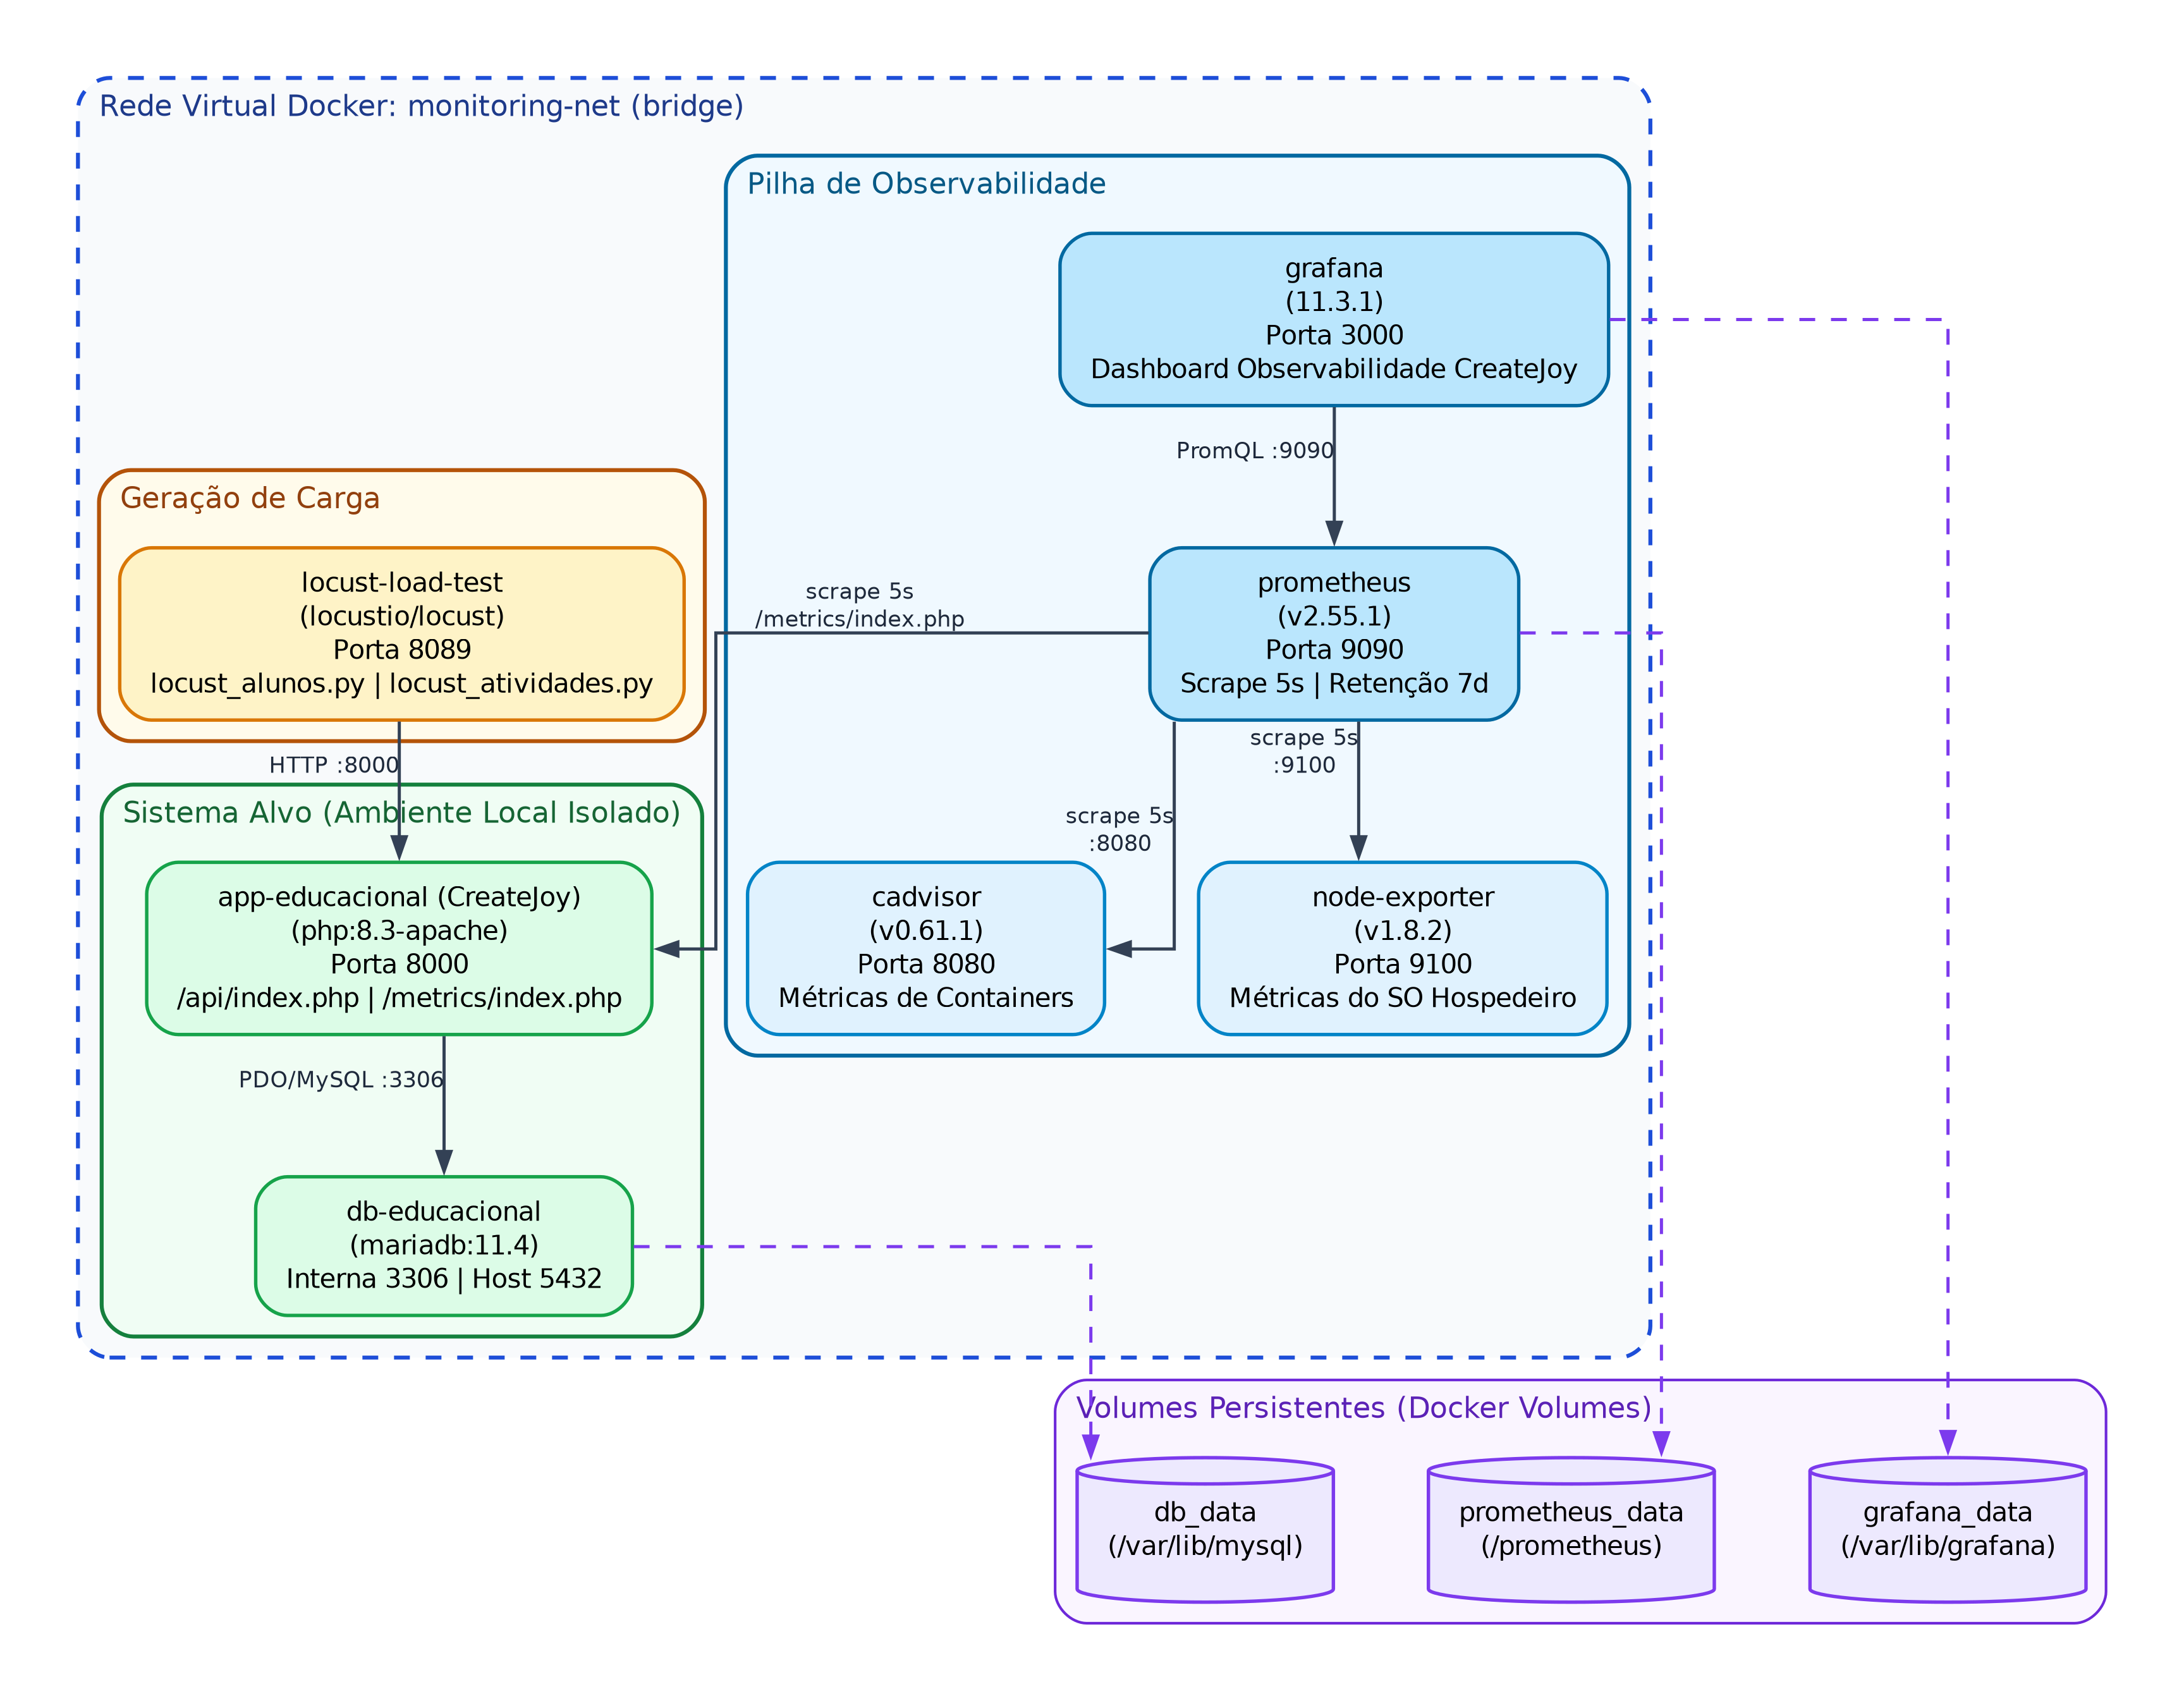
\includegraphics[width=0.92\textwidth]{imagens/arquitetura.png}
    \caption{Arquitetura da solução orquestrada via Docker Compose, destacando a rede virtual \texttt{monitoring-net}, os sete containers integrados, o fluxo de coleta do Prometheus e os três volumes persistentes.}
    \label{fig:arquitetura}
\end{figure*}

Para garantir a ordem correta de inicialização, o serviço \texttt{db} define um \textit{healthcheck} executado a cada 5 segundos com o utilitário \texttt{mariadb-admin ping}. O container \texttt{app} inicia somente após \texttt{db} atingir o estado saudável (\texttt{service\_healthy}) e expõe seu próprio \textit{healthcheck} via requisição HTTP em \texttt{/api/index.php?route=health}. Tanto o \texttt{prometheus} quanto o \texttt{locust} aguardam a disponibilidade saudável de \texttt{app}, evitando falhas prematuras de coleta ou de autenticação durante a subida do ambiente.

A Tabela~\ref{tab:servicos} resume os containers configurados, suas imagens oficiais, o mapeamento de portas e os volumes associados.

\begin{table*}[t]
\centering
\caption{Mapeamento dos containers, imagens, portas e armazenamento persistente na arquitetura.}
\label{tab:servicos}
\begin{tabular}{@{}llllp{4.3cm}@{}}
\toprule
\textbf{Serviço} & \textbf{Imagem / Build} & \textbf{Porta (Host:Container)} & \textbf{Volume} & \textbf{Função Principal} \\
\midrule
\texttt{app} & \texttt{php:8.3-apache} (\texttt{./app}) & \texttt{8000:8000} & Nenhum (stateless) & API PHP e interface web do CreateJoy; expõe \texttt{/metrics/index.php}. \\
\texttt{db} & \texttt{mariadb:11.4} & \texttt{5432:3306} & \texttt{db\_data} & Banco relacional inicializado com esquema, migrações e dados fictícios. \\
\texttt{cadvisor} & \texttt{ghcr.io/google/cadvisor:v0.61.1} & \texttt{8080:8080} & Montagens RO do host & Coleta CPU, RAM, disco e rede de cada container Docker. \\
\texttt{node-exporter} & \texttt{prom/node-exporter:v1.8.2} & \texttt{9100:9100} & \texttt{/proc}, \texttt{/sys}, \texttt{/} (RO) & Expõe métricas de hardware e núcleo do SO hospedeiro. \\
\texttt{prometheus} & \texttt{prom/prometheus:v2.55.1} & \texttt{9090:9090} & \texttt{prometheus\_data} & Banco de séries temporais com coleta a cada 5 s e retenção de 7 dias. \\
\texttt{grafana} & \texttt{grafana/grafana:11.3.1} & \texttt{3000:3000} & \texttt{grafana\_data} & Painéis visuais provisionados automaticamente via código. \\
\texttt{locust} & \texttt{locustio/locust:latest} & \texttt{8089:8089} & \texttt{./load-tests} (RO) & Geração de carga concorrente em Python contra \texttt{http://app:8000}. \\
\bottomrule
\end{tabular}
\end{table*}

Três volumes nomeados garantem persistência entre reinicializações de containers: \texttt{db\_data} armazena os arquivos de dados do MariaDB em \texttt{/var/lib/mysql}; \texttt{prometheus\_data} preserva o banco de séries temporais (TSDB) em \texttt{/prometheus} com janela de retenção configurada para 7 dias; e \texttt{grafana\_data} mantém o estado interno do Grafana em \texttt{/var/lib/grafana}. Na primeira inicialização do banco, cinco scripts SQL montados em modo somente leitura em \texttt{/docker-entrypoint-initdb.d/} criam o esquema completo do CreateJoy, aplicam migrações de negócio e inserem usuários, produtos e missões fictícias (\texttt{seed-demo.sql}).

\section{Tecnologias Utilizadas}

Cada componente foi selecionado para atender a uma responsabilidade isolada no fluxo de observabilidade e geração de carga.

\subsection{Docker e Docker Compose}
O Docker fornece o isolamento de processos e de sistema de arquivos dos serviços, enquanto o Docker Compose~\cite{dockercompose} centraliza a declaração da topologia, das variáveis de ambiente, das dependências de inicialização e dos volumes em um manifesto versionável. Essa abordagem assegura que qualquer integrante do grupo reproduza o mesmo ambiente com o comando \texttt{docker compose up -d --build}.

\subsection{CreateJoy (PHP 8.3/Apache) e MariaDB 11.4}
O sistema alvo é uma réplica local da plataforma educacional CreateJoy, empacotada a partir da imagem \texttt{php:8.3-apache} com a extensão \texttt{pdo\_mysql} e os módulos \texttt{headers} e \texttt{rewrite} habilitados, escutando na porta \texttt{8000}. A persistência é atendida pelo MariaDB 11.4~\cite{mariadb}, escolhido por compatibilidade direta com o esquema relacional da aplicação. A API centraliza as rotas em \texttt{/api/index.php}, empregando cookie de sessão (\texttt{CREATEJOYSESSID}) e proteção contra falsificação de requisição entre sites mediante cabeçalho \texttt{X-CSRF-Token} nas operações de escrita.

Além das rotas de negócio, a aplicação disponibiliza o endpoint \texttt{/metrics/index.php} no formato de exposição de texto do Prometheus. A cada consulta, o script verifica a conectividade com o banco e exporta cinco métricas do tipo \textit{gauge}: \texttt{createjoy\_up}, \texttt{createjoy\_students\_total}, \texttt{createjoy\_pending\_submissions}, \texttt{createjoy\_pending\_store\_requests} e \texttt{createjoy\_metrics\_generation\_seconds}.

\subsection{cAdvisor e Node Exporter}
O cAdvisor~\cite{cadvisor} (versão \texttt{v0.61.1}) executa em modo privilegiado com acesso somente leitura a \texttt{/rootfs}, \texttt{/var/run}, \texttt{/sys}, \texttt{/var/lib/docker} e \texttt{/dev/disk}, coletando métricas de uso de CPU, conjunto de trabalho de memória (\textit{working set}), leitura e escrita em sistema de arquivos e tráfego de rede por container. O Node Exporter~\cite{nodeexporter} (versão \texttt{v1.8.2}) monta \texttt{/proc}, \texttt{/sys} e a raiz do sistema em modo somente leitura para reportar os contadores globais do SO hospedeiro, excluindo pontos de montagem virtuais pela expressão regular configurada em \texttt{--collector.filesystem.mount-points-exclude}.

\subsection{Prometheus}
O Prometheus~\cite{prometheus} (versão \texttt{v2.55.1}) atua como coletor ativo (\textit{pull model}) e banco de séries temporais. O arquivo \texttt{prometheus/prometheus.yml} define \texttt{scrape\_interval} e \texttt{evaluation\_interval} de 5 segundos, com \texttt{scrape\_timeout} de 4 segundos, permitindo resposta visual rápida durante a demonstração ao vivo. Quatro alvos (\textit{jobs}) são monitorados: \texttt{prometheus} (\texttt{localhost:9090}), \texttt{cadvisor} (\texttt{cadvisor:8080}), \texttt{node-exporter} (\texttt{node-exporter:9100}) e \texttt{createjoy-app} (\texttt{app:8000/metrics/index.php}).

\subsection{Grafana}
O Grafana~\cite{grafana} (versão \texttt{11.3.1}) provê a interface gráfica de visualização. Tanto a fonte de dados (\texttt{datasource.yml}, apontando para \texttt{http://prometheus:9090}) quanto o painel \textit{Observabilidade CreateJoy} (\texttt{observabilidade-so.json}) são carregados por provisionamento declarativo em \texttt{grafana/provisioning/}. O painel reúne dez visualizações com atualização automática a cada 5 segundos: quatro cartões de estado (CPU do host, Memória RAM do host, disponibilidade da aplicação via \texttt{createjoy\_up} e entregas pendentes via \texttt{createjoy\_pending\_submissions}) e seis séries temporais (CPU por container, Memória RAM por container, I/O de disco do host, Tráfego de rede do host, I/O de disco por container e Tráfego de rede por container).

\subsection{Locust (Python em Container)}
O Locust~\cite{locust} executa integralmente dentro do container \texttt{locustio/locust:latest}, dispensando a instalação de interpretadores ou bibliotecas no hospedeiro. Ele permite definir o comportamento de usuários virtuais em Python e controlar dinamicamente o número de usuários simultâneos e a taxa de entrada (\textit{ramp-up}) pela interface web na porta \texttt{8089} ou em modo \textit{headless} via terminal.

\section{Execução e Validação Experimental}

\subsection{Delineamento Experimental e Cenários de Carga}
A validação experimental foi estruturada em três etapas sequenciais: observação do sistema em estado ocioso para obtenção da linha de base (\textit{baseline}), execução do Cenário~1 (navegação e compras simultâneas) e execução do Cenário~2 (envio simultâneo de atividades com entradas de tamanhos variados). Para padronizar a coleta em qualquer máquina com Docker ativo, foi incluído no repositório o script auxiliar \texttt{monitoramento/coletar\_evidencias.sh}.

No Cenário~1 (\texttt{load-tests/locust\_alunos.py}), cada usuário virtual autentica com a conta fictícia \texttt{aluno.demo@createjoy.local} em \texttt{POST /api/index.php?route=auth/login}, armazena o cookie de sessão e o token \texttt{X-CSRF-Token}, e executa tarefas com intervalo de espera aleatório entre 0,5~s e 2,0~s seguindo pesos proporcionais:
\begin{itemize}
    \item \textbf{Consulta ao painel do aluno (peso 4):} requisição \texttt{GET /api/index.php?route=bootstrap}.
    \item \textbf{Abertura do catálogo da CreateStore (peso 3):} requisição \texttt{GET /api/index.php?route=bootstrap}.
    \item \textbf{Solicitação de produto na loja (peso 1):} requisição \texttt{POST} na rota \texttt{store/request/create} de \texttt{/api/index.php}, com seleção aleatória de produto e envio do cabeçalho CSRF.
\end{itemize}

No Cenário~2 (\texttt{load-tests/locust\_atividades.py}), cada usuário virtual autentica, identifica missões ativas disponíveis para o perfil e submete arquivos de código Arduino (\texttt{.ino}) via \texttt{POST /api/index.php?route=submissions/create} em formato \texttt{multipart/form-data}. Os conteúdos são pré-gerados em memória antes do início das requisições para evitar sobrecarga de CPU no próprio container do Locust. A variável de ambiente \texttt{TAMANHO\_ENTRADA} permite isolar ou combinar três portes de entrada:
\begin{itemize}
    \item \textbf{Entrada pequena (1~KB, peso 3):} um arquivo \texttt{sketch\_1kb.ino}, voltado à medição da sobrecarga mínima de requisição.
    \item \textbf{Entrada média (100~KB, peso 2):} um arquivo \texttt{sketch\_100kb.ino}, exercitando serialização, escrita moderada em disco e tráfego de rede.
    \item \textbf{Entrada grande (5~MB totais, peso 1):} dividida em três anexos \texttt{files[]} de aproximadamente 1,67~MB cada, respeitando o limite padrão \texttt{upload\_max\_filesize=2M} do PHP/Apache e o teto de 8~MB por tentativa definido pela aplicação.
\end{itemize}

As consultas PromQL utilizadas no painel \textit{Observabilidade CreateJoy} para capturar o comportamento do sistema são:
\begin{itemize}
    \item \textbf{CPU do host (\%):}\\
    {\footnotesize\texttt{100 - (avg(rate(node\_cpu\_seconds\_total}}\\
    {\footnotesize\texttt{\{mode="idle"\}[1m])) * 100)}}
    \item \textbf{CPU por container (\%):}\\
    {\footnotesize\texttt{sum by (name) (rate(container\_cpu\_usage}}\\
    {\footnotesize\texttt{\_seconds\_total\{name!=""\}[1m])) * 100}}
    \item \textbf{Memória RAM do host (\%):}\\
    {\footnotesize\texttt{(1 - (node\_memory\_MemAvailable\_bytes /}}\\
    {\footnotesize\texttt{node\_memory\_MemTotal\_bytes)) * 100}}
    \item \textbf{Memória RAM por container (bytes):}\\
    {\footnotesize\texttt{sum by (name) (container\_memory\_working}}\\
    {\footnotesize\texttt{\_set\_bytes\{name!=""\})}}
    \item \textbf{I/O de disco e rede:} taxas de leitura e escrita (\texttt{node\_disk\_*}, \texttt{container\_fs\_*}) e recepção/transmissão (\texttt{node\_network\_*}, \texttt{container\_network\_*}) em janela de 1 minuto.
\end{itemize}

\subsection{Estado Base (Sistema Ocioso)}
Antes da injeção de carga, confirma-se por \texttt{docker compose ps} que \texttt{app-educacional} e \texttt{db-educacional} encontram-se no estado \texttt{healthy}, enquanto os quatro alvos do Prometheus (\texttt{prometheus}, \texttt{cadvisor}, \texttt{node-exporter} e \texttt{createjoy-app}) aparecem como \texttt{UP} em \texttt{http://localhost:9090/targets}. Com a plataforma ociosa, a métrica \texttt{createjoy\_up} permanece igual a 1 e os gráficos de CPU, memória, disco e rede registram apenas o custo basal dos processos em espera e dos ciclos de coleta de 5 segundos.

\noindent\textbf{[PENDENTE:} Inserir captura de tela do comando \texttt{docker compose ps}, da página \texttt{/targets} do Prometheus com os 4 alvos \texttt{UP} e do dashboard \textit{Observabilidade CreateJoy} em estado ocioso, salvando as imagens em \texttt{relatorio/imagens/}\textbf{].}

\subsection{Cenário 1: Usuários Simultâneos e Compras na Loja}
A execução progressiva de \texttt{locust\_alunos.py} (por exemplo, patamares de 10, 50 e 100 usuários virtuais) permite verificar como o aumento de concorrência altera o tempo de resposta mediano, o percentil 95 (\textit{p95}) e a taxa de falhas reportados pelo Locust, correlacionando tais variações aos picos de CPU nos containers \texttt{app-educacional} e \texttt{db-educacional} e ao aumento do contador \texttt{createjoy\_pending\_store\_requests}.

\noindent\textbf{[PENDENTE:} Preencher a Tabela~\ref{tab:resultados} e inserir captura de tela do Grafana e da aba \textit{Statistics} do Locust durante a execução de \texttt{locust\_alunos.py} em ambiente com Docker ativo\textbf{].}

\subsection{Cenário 2: Envio Simultâneo de Atividades com Entradas Variadas}
A execução isolada dos modos \texttt{pequeno} (1~KB), \texttt{medio} (100~KB) e \texttt{grande} (5~MB) em \texttt{locust\_atividades.py} expõe a diferença de pressão sobre os subsistemas do SO: envios de 1~KB concentram o custo no processamento HTTP/PHP e nas inserções de metadados no MariaDB, enquanto envios de 5~MB elevam simultaneamente o tráfego de rede na ponte \texttt{monitoring-net}, o consumo de memória temporária do Apache/PHP durante o recebimento \textit{multipart}, o cálculo de hash de integridade e a taxa de escrita em disco no diretório \texttt{storage/uploads}.

\begin{table*}[t]
\centering
\caption{Consolidação planejada das métricas experimentais coletadas no Grafana e no Locust.}
\label{tab:resultados}
\begin{tabular}{@{}lcccccc@{}}
\toprule
\textbf{Cenário} & \textbf{Usuários} & \textbf{CPU Host (\%)} & \textbf{CPU App / DB (\%)} & \textbf{RAM App (MB)} & \textbf{Escrita Disco (B/s)} & \textbf{Latência p95 (ms)} \\
\midrule
Ocioso (Baseline) & 0 & [PENDENTE] & [PENDENTE] & [PENDENTE] & [PENDENTE] & N/A \\
Alunos e Loja (Baixa) & 10 & [PENDENTE] & [PENDENTE] & [PENDENTE] & [PENDENTE] & [PENDENTE] \\
Alunos e Loja (Média) & 50 & [PENDENTE] & [PENDENTE] & [PENDENTE] & [PENDENTE] & [PENDENTE] \\
Alunos e Loja (Alta) & 100 & [PENDENTE] & [PENDENTE] & [PENDENTE] & [PENDENTE] & [PENDENTE] \\
Atividades (1 KB) & 20 & [PENDENTE] & [PENDENTE] & [PENDENTE] & [PENDENTE] & [PENDENTE] \\
Atividades (100 KB) & 20 & [PENDENTE] & [PENDENTE] & [PENDENTE] & [PENDENTE] & [PENDENTE] \\
Atividades (5 MB) & 20 & [PENDENTE] & [PENDENTE] & [PENDENTE] & [PENDENTE] & [PENDENTE] \\
\bottomrule
\end{tabular}
\end{table*}

\noindent\textbf{[PENDENTE:} Inserir capturas de tela comparativas do Grafana para os envios de 1~KB, 100~KB e 5~MB evidenciando a variação de Memória RAM, I/O de disco, Tráfego de rede e incremento em \texttt{createjoy\_pending\_submissions}\textbf{].}

\subsection{Análise de Contenção de Recursos do SO e Limitações}
A separação entre métricas do hospedeiro (Node Exporter) e métricas por container (cAdvisor) esclarece quatro fenômenos clássicos de sistemas operacionais sob carga:
\begin{itemize}
    \item \textbf{Contenção de CPU:} múltiplas requisições PHP concorrentes e consultas simultâneas ao MariaDB aumentam a fila de processos prontos (\textit{run queue}) no escalonador do núcleo. Em máquinas multinúcleo, o percentual de CPU por container reportado pelo cAdvisor pode ultrapassar 100\%, pois cada 100\% equivale à saturação de um núcleo lógico.
    \item \textbf{Pressão de Memória:} o conjunto de trabalho (\texttt{container\_memory\_working\_set\_bytes}) cresce com o número de \textit{workers} ativos do Apache/PHP e com o tamanho dos buffers de requisição \textit{multipart}. Retenção elevada após o término do teste sinaliza cache não liberado ou pressão para troca em disco (\textit{swap}).
    \item \textbf{Contenção de I/O de Disco:} operações simultâneas de escrita de transações no MariaDB e gravação de anexos \texttt{.ino} em \texttt{storage/uploads} disputam a largura de banda do dispositivo de armazenamento, elevando a latência de cauda (\textit{p95} e \textit{p99}).
    \item \textbf{Tráfego de Rede Virtual:} a troca de pacotes entre \texttt{locust}, \texttt{app} e \texttt{db} atravessa a pilha de rede do núcleo via interfaces virtuais (\textit{veth}) ligadas à ponte \texttt{monitoring-net}, somando custo de cópia de buffers em memória e interrupções de software.
\end{itemize}

Como limitação metodológica conhecida, quando o ambiente executa em Docker Desktop sobre Windows com WSL~2, as métricas reportadas pelo Node Exporter refletem a máquina virtual Linux interna gerenciada pelo WSL~2, e não os contadores nativos completos do sistema hospedeiro Windows. Adicionalmente, o fato de o container gerador de carga (\texttt{locust}) compartilhar o mesmo hospedeiro da aplicação faz com que parte do consumo global de CPU e rede observado no Node Exporter provenha do próprio gerador de testes, o que torna a discriminação por container fornecida pelo cAdvisor indispensável na interpretação dos resultados.

\section{Conclusão}

A arquitetura desenvolvida integra uma aplicação web real em ambiente isolado a uma pilha completa de observabilidade baseada em Prometheus, Grafana, cAdvisor e Node Exporter, orquestrada de forma declarativa em Docker Compose. A inclusão de um endpoint próprio de métricas no CreateJoy (\texttt{/metrics/index.php}) em conjunto com os agentes de infraestrutura permite cruzar indicadores de negócio, como entregas e solicitações pendentes, com contadores de baixo nível do sistema operacional.

Os scripts de carga em Python com Locust oferecem controle reproduzível tanto sobre a concorrência de usuários quanto sobre o porte das entradas enviadas ao servidor, possibilitando evidenciar a contenção de CPU, memória RAM, I/O de disco e rede em tempo real. Como trabalhos futuros concretos, destacam-se a definição de limites explícitos de CPU e memória por container (\texttt{deploy.resources.limits}) no Docker Compose para estudar o comportamento de \textit{throttling} e de término por falta de memória (OOM Killer), bem como a execução do gerador de carga em um hospedeiro fisicamente separado para eliminar a interferência do Locust nas métricas globais do Node Exporter.

\section{Repositório}

Os manifestos de orquestração (\texttt{docker-compose.yml}), a configuração do Prometheus (\texttt{prometheus/prometheus.yml}), o provisionamento e o painel JSON do Grafana (\texttt{grafana/provisioning/}), os scripts de teste de carga (\texttt{load-tests/}), o script de coleta automatizada (\texttt{monitoramento/coletar\_evidencias.sh}), o código da aplicação local (\texttt{app/}) e o código-fonte em \LaTeX{} deste relatório estão disponíveis no repositório oficial da equipe:

\begin{itemize}
    \item \textbf{GitHub:} \url{https://github.com/1g0rX/trabalho-pratico-sistemas-distribuidos}
\end{itemize}

\begin{thebibliography}{00}
\bibitem{dockercompose} Docker Inc., ``Docker Compose Documentation,'' Disponível em: \url{https://docs.docker.com/compose/}.
\bibitem{mariadb} MariaDB Foundation, ``MariaDB Server Documentation,'' Disponível em: \url{https://mariadb.com/kb/en/documentation/}.
\bibitem{cadvisor} Google, ``cAdvisor (Container Advisor),'' Disponível em: \url{https://github.com/google/cadvisor}.
\bibitem{nodeexporter} Prometheus Authors, ``Node Exporter,'' Disponível em: \url{https://github.com/prometheus/node_exporter}.
\bibitem{prometheus} Prometheus Authors, ``Prometheus Documentation,'' Disponível em: \url{https://prometheus.io/docs/}.
\bibitem{grafana} Grafana Labs, ``Grafana Documentation,'' Disponível em: \url{https://grafana.com/docs/}.
\bibitem{locust} Locust Authors, ``Locust Documentation,'' Disponível em: \url{https://docs.locust.io/}.
\end{thebibliography}

\end{document}
